\documentclass{article}

% packages
\usepackage[skip=10pt, indent=40pt]{parskip}
\usepackage{geometry}
\geometry{
  a4paper,
  total={170mm, 257mm},
  left=20mm,
  top=20mm
}
\usepackage{graphicx}
\graphicspath{{./images/}}
% renew commands
\renewcommand{\labelenumii}{\roman{enumii}}

% define title
\title{%
  CMSC 124 Final Project\\
  \large 
}
\author{
  delCastillo, Kyle Adrian
  \and
  Pareja, King John
}


% document start
\begin{document}
\maketitle

\section*{Python}

\subsection*{Purpose (Intended use) and Motivations}
Python is a high-level, dynamically-typed, interpreted programming language. It is designed to be readable, easy to learn, and simple to use. Python was originally developed as a bridge between shell-scripting (bash) and C, and today it has been extended to have multiple capabilities.

\subsection*{History (Authors, Revisions, Adoption)}
Originally developed by Guido Van Rossum in 1989, it was intended as a scripting language between bash-scripting and C
but more easily programmable than C and more readable than shell scripts. It was named after Monty Python, a british comedy troupe. \par
In February 1991, Van Rossum published the source code of Python’s interpreter to alt.sources, a Usenet group for open-source code. The first release (0.9.0) had features such as classes, exception handling, functions, core datatypes like list, dict, str, and so on. In January 1994, version 1.0 was released and Guido was later invited to the USA by the US National Institute for Standards and Technology to develop further releases of python. Python 2.0 released in October 2000 with list comprehensions which was then present in programming languages like Haskell, with other additional features like unicode support and a full garbage collector. 
\par The Python Software Foundation was established in March 6 2001, taking over the development of the core Python distribution, managing intellectual rights, developer conferences, and raising funds. In December 2008, Python 3.0 was released, leading to the retirement of continuous updates for Python 2.x on 2020 as many codebases that relied on older versions of Python were slowly translated to Python 3. Today, the latest stable version of Python is 3.11.
\begin{figure}[ht]
  \centering
  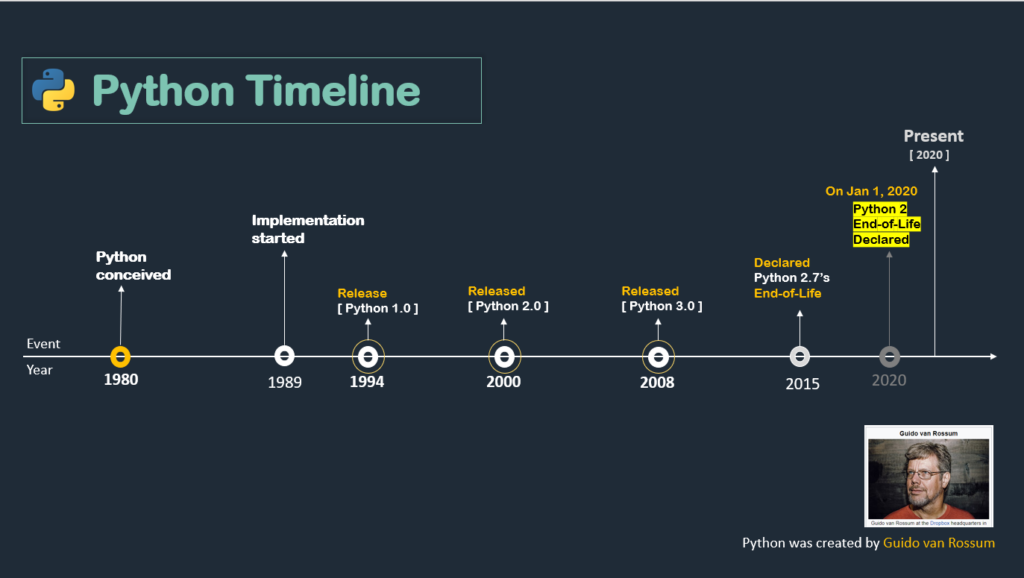
\includegraphics[width=0.8\textwidth]{py_history}
  \caption{Timeline of Python history with milestones (aipython, 2019)}
\end{figure}
\newpage
\subsection*{Language Features}
Python is a high-level, general-purpose programming language that has a wide range of features that make it well-suited for many types of projects. Some of the main features of Python include:
\begin{enumerate}
  \item Easy to learn and use
    \subitem Python has a simple and easy-to-learn syntax, which makes it an ideal language for beginners. It also has a large and active community, which means that there are many resources available for learning and using Python.
  \item High-level datatypes 
    \subitem Python includes built-in support for many high-level data types, such as lists, dictionaries, and sets, which makes it easy to store and manipulate complex data.
  \item Object-oriented programming
    \subitem Python supports object-oriented programming (OOP), which is a programming paradigm that is based on the concept of "objects", which can contain data and code that manipulates that data. In Python, you can use OOP by defining classes, which are templates for creating objects.
  \item Large standard library
    \subitem Python has a large standard library, which means that there are many pre-written modules and functions that you can use in your code. This makes it easy to perform common tasks, such as connecting to a database or reading and writing files.
  \item Dynamically-typed 
    \subitem Python is a dynamically-typed language, which means that you don't have to specify the type of a variable when you declare it. This makes it easy to write code quickly, but it can also make it harder to find certain types of errors.
  \item Interpreted
    \subitem Python is an interpreted language, which means that it is not compiled to machine code before it is executed. Instead, it is interpreted by another program at runtime. This makes it easy to run Python code on any system that has an interpreter, but it can also make the code run slower than compiled languages.
\end{enumerate}

\subsection*{Paradigm(s)}
There are several programming paradigms that are supported by Python, including object-oriented programming, imperative programming, and functional programming

\begin{itemize}
  \item Object-oriented programming (OOP)
    \subitem A programming paradigm that is based on the concept of "objects", which can contain data and code that manipulates that data. In Python, you can use OOP by defining classes, which are templates for creating objects. Objects are instances of classes and they can have attributes (data) and methods (functions that manipulate the data).
  \item Imperative programming
    \subitem A programming paradigm that is based on the idea of giving the computer a sequence of tasks to perform, using statements that change a program's state. In Python, you can use imperative programming by writing statements that manipulate variables and control the flow of the program.
  \item Functional Programming 
    \subitem A programming paradigm that is based on the idea of treating computation as the evaluation of mathematical functions. In Python, you can use functional programming by writing functions that take input and return output, without modifying any state.
\end{itemize}

Python is considered to be a \emph{multiparadigm} language because it supports multiple programming paradigms. This means that you can use Python to write code in different styles, depending on your needs and preferences. For example, you can use Python to write object-oriented code, or you can use it to write functional code. This flexibility makes Python a popular choice for many types of projects.
\subsection*{Language Evaluation Criteria}
\begin{itemize}
  \item Readability
    \subitem Python is known for its readable, clean syntax. It uses indentation to indicate code blocks, rather than curly braces like many other languages. This makes Python code easy to read and understand, as it follows a natural, logical structure. Python's large standard library with clear, concise documentation, further improves readability.
  \item Writability
    \subitem Python is a dynamically-typed language, which means that you do not need to specify the type of a variable when you declare it. This can make Python code easier to write, as you do not need to spend time declaring variable types. Python's large standard library and downloadable third-party libraries provide many pre-built functions and classes that you can use in your code. This can help to reduce the amount of code you need to write and improve your productivity.
  \item Reliability 
    \subitem Python is a robust and reliable language. It has a strong exception-handling system, which helps to prevent errors and bugs from crashing your program. Python also has a large and active user community, which means that there is a wealth of support and resources available if you encounter any issues.
\end{itemize}

Overall, Python's readable, writable, and reliable nature make it a popular choice for many types of projects, including web development, data analysis, and scientific computing. 
\section*{R}
\subsection*{Purpose (Intended use) and Motivations}
R is a programming language is a free software environment mainly used for statistical computing, data analysis, and statistcal graphics. It compiles and runs on a wide variety of UNIX platforms, Windows and MacOS. R was originally developed as a sucessor to the S language, and is now used as a statistical programming language in the field of datamining, bioinformatics, statistics, and data analytics in the development and usage of statistical software.

\subsection*{History (Authors, Revisions, Adoption)}
R has its foundations in the S programming language, originally developed by John CHambers at the Bell Laboratories during the mid 1970s, where the Bell Labs focused their attention on statistical analysis (Becker cited in Giorgi, 2022). 
\subsection*{Language Features}
\subsection*{Paradigm(s)}
\subsection*{Language Evaluation Criteria}

\section*{Feature 1}
\subsection*{Description of feature in Language A not present in B}
\subsection*{Advantages of having the feature}
\subsection*{Advantages of not having the feature}
\subsection*{How to implement similar functionality in B}

\section*{Feature 2}
\subsection*{Description of feature in Language A not present in B}
\subsection*{Advantages of having the feature}
\subsection*{Advantages of not having the feature}
\subsection*{How to implement similar functionality in B}


\end{document}
